\documentclass[12pt, oneside]{article}
\usepackage{geometry}
\usepackage[utf8]{inputenc}
\usepackage{setspace}
\usepackage{times}
\usepackage{url}
\urlstyle{same}
\usepackage{multirow}
\usepackage[usegeometry]{typearea}
% Useful for checking layout
% \usepackage{showframe}
\usepackage{fancyhdr}
\usepackage{blindtext}
% Indenting the first sentence after section
\usepackage{indentfirst}
% Set language
\usepackage[german]{babel}
% Abbreviations
\usepackage{glossaries}
% For big tables which span multiple pages
\usepackage{longtable}
% Images
\usepackage{graphicx}
\graphicspath{ {./images/} }
% APA Citation Style
\usepackage[natbibapa]{apacite}
% Smaller font size for captions
\usepackage[font=small,labelfont=bf]{caption}
% Table related packages
\usepackage{booktabs}


\geometry{
 a4paper,
 left=30mm,
 top=25mm,
 right=25mm,
 bottom=20mm,
 footskip=15pt,
}

\setstretch{1.3} % Define Line Spacing
\renewcommand{\headrulewidth}{0pt} % Remove footer line

\pagestyle{fancy} % Allow for customizing header and footer
% Customize footer for page number location
\fancyhf{}
\fancyfoot{}
\fancyhead[R]{Yannick Hutter}
\fancyhead[L]{Bachelorthesis}
\fancyfoot[R]{\thepage}



 \makeglossaries

 \newglossaryentry{dsr}
 {
     name=DSR,
     description={Design science Research}
 }
 
 \newglossaryentry{covid19}
 {
     name=COVID-19,
     description={Coronavirus-Krankheit-2019 ~\citep{covid19}}
 }
 \newglossaryentry{bfs}
 {
     name=BFS,
     description={Bundesamt für Statistik}
 }
 
 \newglossaryentry{foph}
 {
     name=FOPH,
     description={Federal Office of Public Health}
 }
 \newglossaryentry{fhgr}
 {
     name=FHGR,
     description={Fachhochschule Graubünden}
 }
 \newglossaryentry{svi}
 {
     name=SVI,
     description={Social Vulnerability Index}
 }
 \newglossaryentry{who}
 {
     name=WHO,
     description={World Health Organisation}
 }



\begin{document}
\pagenumbering{roman}
\begin{titlepage}
	\begin{center}
		\Huge
		\textbf{Bachelorthesis}\\
		\vspace{0.5cm}
		\LARGE
		Analyse und Implementierung eines personalisierbaren Corona Dashboards für Millenials

		\vspace{1.5cm}
		\normalsize
		\textbf{Yannick Hutter}\\
		\textbf{Digital Business Management Klasse 18tz}\\
		\textbf{Talackerstrasse 8}\\
		\textbf{8887 Mels}\\
		\textbf{yannick.hutter@stud.fhgr.ch}\\


		\vfill
		Referrent: Daniel Klinkhammer\\
		Korefferent: Michael Burch\\

		\vspace{0.8cm}


		Digital Business Management\\
		Fachhochschule Graubünden\\
		Mels, April 2022
	\end{center}
\end{titlepage}

\clearpage
\section*{Abstract}
TODO


\clearpage
\tableofcontents

\clearpage
\listoffigures
\listoftables

\clearpage
\printglossaries

\pagenumbering{arabic}

\clearpage
\section{Einleitung}
Seit Beginn der Menschheitsgeschichte gab es bereits unzählige Pandemien, welche ihren Tribut gefordert haben. Die neuste Pandemie, auch bekannt unter dem Namen \Gls{covid19}, ist hierbei keine Ausnahme und zählt zu den Spitzenreitern in Bezug auf die tägliche Anzahl krankheitsbedingter Todesfälle nach einer Erkrankung (siehe Abbildung 1).

\begin{figure}[ht]
    \includegraphics[width=12cm]{images/krankheitsbedingte_todesfälle_nach_erkrankung.png}
    \centering
    \caption{Durchschnittliche tägliche Anzahl krankheitsbedingter Todesfälle weltweit nach Erkrankung (Stand:
1. Januar 2021) ~\citep[S. 12]{worldwide_epidemic_cases_study}}
\end{figure}

\Gls{covid19}, fortlaufend als Corona bezeichnet, hat sowohl in den wirtschaftlichen als auch in den sozialen Strukturen tiefgreifende Veränderungen herbeigeführt. Um die Bevölkerung auf die Gefahr der Pandemie zu sensibilisieren und die rasant steigenden Fallzahlen (siehe Abbildung 2) des Virus einzudämmen, wurden diverse Anstrengungen unternommen.

\begin{figure}[ht]
    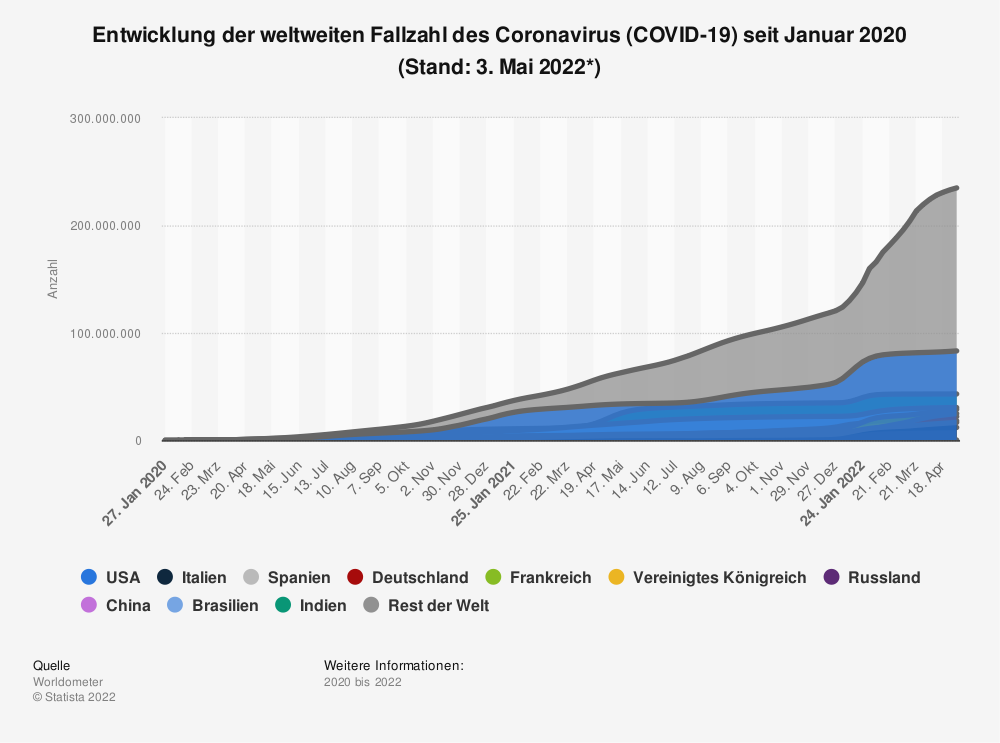
\includegraphics[width=10cm]{images/corona_fallzahlen.png}
    \centering
    \caption{Entwicklung der weltweiten Fallzahl des Coronavirus (COVID-19) seit Januar 2020 ~\citep{covid_cases_worldwide}}
\end{figure}

Eine zentrale Rolle spielten hierbei \textit{Datenvisualisierungen}. Wichtig in diesem Kontext zu verstehen ist, dass sich der Begriff Datenvisualisierungen nicht nur aus Linien- oder Kuchendiagrammen definiert, sondern ein breites Spektrum von verschiedenen Visualisierungen, darunter auch Infografiken, abdeckt. So erstellte zum Beispiel das \Gls{bfs} diverse Infografiken in den Bereichen Gesundheit, Kultur sowie Kriminalität, in Bezug auf Corona ~\citep{covid19_bfs_infografiken}.

Besonders während einer weltweiten Pandemie wie Corona ist eine akkumulierte Sicht von verschiedenen Visualisierungsarten von zentraler Bedeutung. Dies kann mit Hilfe von \textit{Dashboards} bewerkstelligt werden. Der Begriff Dashboard kommt ursprünglich aus dem Englischen und bezieht sich auf das Armaturenbrett des Autos, wo alle relevanten Informationen übersichtlich auf einem Blick sichtbar sind ~\citep{Duden.18.04.2022}. In Bezug auf Corona werden auf Dashboards unter anderem wichtige Informationen wie Ansteckungszahlen und Todesfälle visualisiert. Ein Beispiel für ein Dashboard ist das \textit{WHO Coronavirus Dashboard}, welches von der \Gls{who} erstellt wurde ~\citep{who_dashboard}. Dass nebst dem in der Schweiz angesiedelten BFS selbst eine weltweite Organisation wie WHO sich um die Erstellung von Dashboards zur Corona Thematik bemüht, soll aufzeigen wie wichtig Datenvisualisierungen und insbesondere Dashboards geworden sind.

\subsection{Kontextabgrenzung}
Die vorliegende Arbeit befasst sich mit Datenvisualisierungen, welche im Zuge der Corona-Pandemie erstellt worden sind. Jedoch wird der Hauptfokus der vorliegenden Arbeit gezielt auf \textbf{Corona-Dashboards} gelegt. Zum Einen erlauben Dashboards die \textit{Kombination} von verschiedenen Datenvisualisierungen, zum Anderen erlauben sie eine akummulierte Sicht auf die \textit{relevantesten Informationen} für eine bestimmte Zielgruppe. Die Wichtigkeit von Dashboards haben auch weltweite Regierungsorganisationen erkannt. Gemäss Barbazza war das \textit{webbasierte Dashboards} die bevorzugte Visualisierungsart von Regierungsorganisationen, wenn es darum geht, Informationen zur Corona-Pandemie darzustellen ~\citep{Barbazza.}.

\subsection{Stand der Forschung}
 Die Coronavirus-Pandemie greift seit ihrem Aufkommen im Jahr 2019 in eine Vielzahl von Lebensbereichen ein. Es ist wenig verwunderlich, dass zu einem solch einschneidendem Thema eine grosse Anzahl von wissenschaftlichen Publikationen erstellt worden sind. Nachfolgend wird auf die wichtigsten bereits bestehenden Studien eingegangen, welche sich mit Corona Datenvisualisierungen sowie mit Dashboards im Allgemeinen beschäftigen.
 
 \subsubsection{Die Landschaft der Corona Datenvisualisierungen}
 Eine massgebende Studie um einen Überblick über die \textit{Landschaft der Corona Datenvisualisierungen} zu erhalten, ist die Studie von Zhang. Bei dieser Studie wurden rund 668 Corona Datenvisualisierungen im Zeitraum vom 22. Januar bis zum 31. Juli 2020 analysiert. Ein wichtiges Auswahlkriterium bei diesen Visualisierungen war, dass die allgemeine Bevölkerung als Zielgruppe im Fokus stand. Anschliessend wurden diese Visualisierungen sowohl mittels \textit{deduktiver} als auch \textit{induktiver} Codierung in Form eines Codebooks zusammengefasst ~\citep[S. 3]{YixuanZhang.}. Aus dem erstellten Codebook sind ebenfalls verschiedene \textit{Nachrichtenkategorien} sowie die dazugehörigen \textit{Visualisierungsarten} ersichtlich. Eine Nachrichtenkategorie beschreibt hierbei die Intention der Datenvisualisierungen (zum Beispiel Information über den Schweregrad der Pandemie). Unter die Kateogrie Visualisierungsarten fallen zum Beispiel Liniendiagramme etc. Beim Erstellen des Codebooks wurde zudem ein \textit{konzeptionelles Framework zum Verständnis von Datenvisualisierungen in Krisenzeiten} erstellt (siehe Abbildung 3). Die Studie von Zhang fokusierte sich hierbei primär auf die ersten drei Aspekte des Models (\textit{who uses what data to communicate what message in what form}). 
 
 \begin{figure}[ht]
    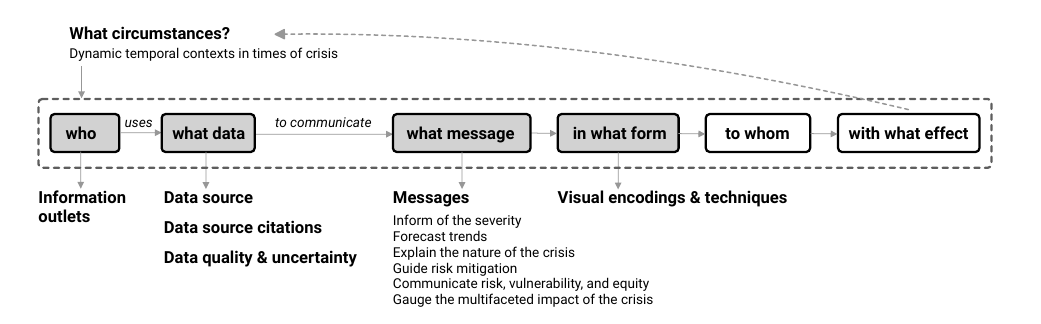
\includegraphics[width=12cm]{images/zhang_conceptual_framework.png}
    \centering
    \caption{Konzeptionelles Framework zum Verständnis von Datenvisualisierungen in Krisenzeiten ~\citep[S. 4]{YixuanZhang.}}
\end{figure}
 
\subsubsection{Corona-Dashboards}
Während der Corona Pandemie sind eine Vielzahl von Dashboards angefertigt worden. Eine interessante Studie in diesem Zusammenhang ist die Studie von Ivankovic ~\citep{Ivankovic.2021}. Diese Studie untersuchte im Speziellen \textit{webbasierte Dashboards}. Konkret wurden hierbei Aspekte wie Funktion (Purpose), Inhalt und Daten (What) sowie die eigentliche Visualisierung (how they communicate COVID-19 data) untersucht. Aus den insgesamt 158 untersuchten Dashboards wurden anschliessend die Gemeinsamkeiten evaluiert. Hieraus entstanden anschliessend 7 zentrale Merkmale von webbasierten Dashboards (siehe Abbildung 4). Diese Merkmale bildeten anschliessend die Grundlage, um die 158 untersuchten Dashboards zu bewerten.
\clearpage

 \begin{figure}[ht]
    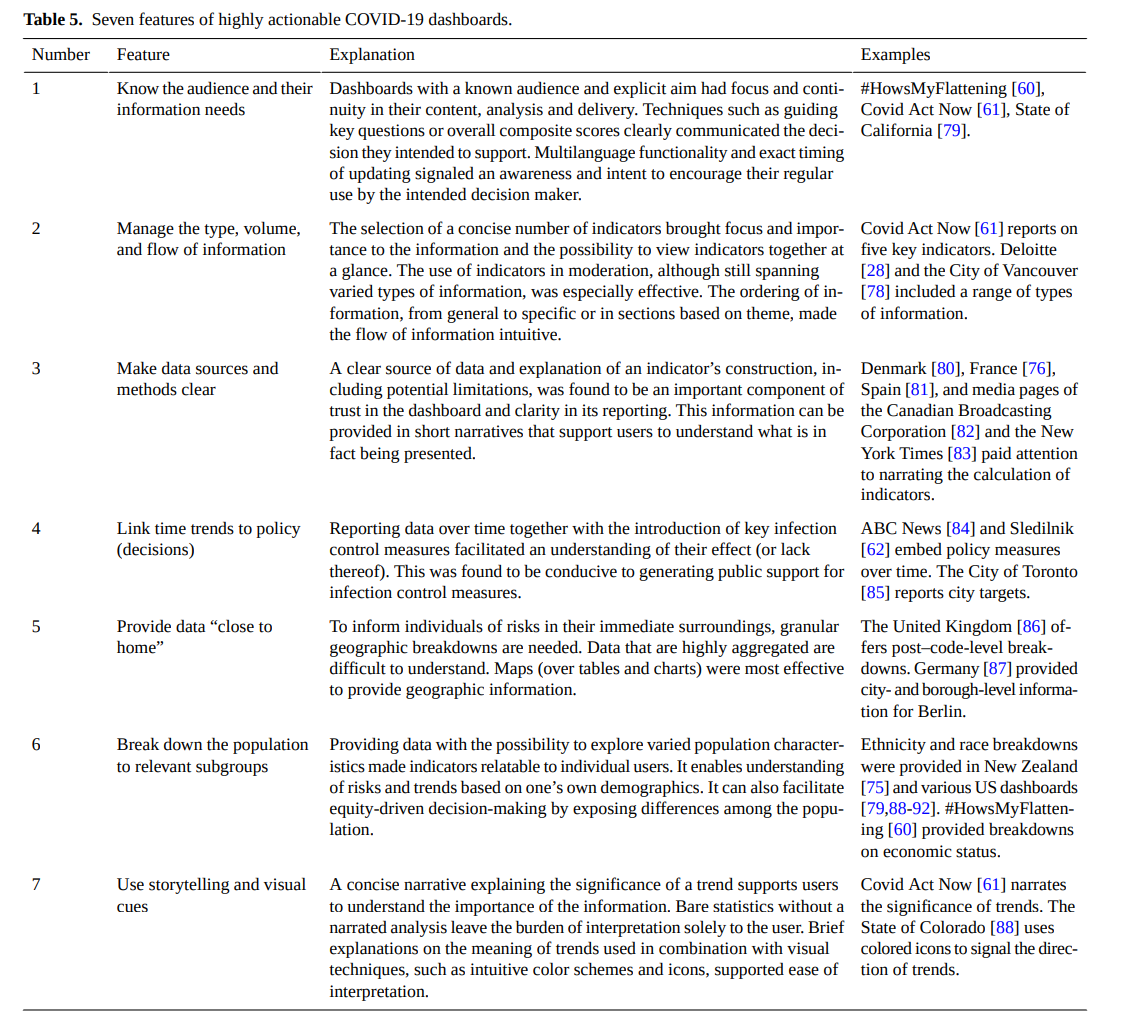
\includegraphics[width=10cm]{images/ivankovic_dashboard_characteristics.png}
    \centering
    \caption{Merkmale von webbasierten Dashboards gemäss Ivankovic ~\citep[S. 12]{Ivankovic.2021}}
\end{figure}


Es gibt aber auch Studien welche Corona-Dashboards aus dem Blickwinkel der Ersteller betrachten. Die Studie von Barbazza untersuchte die gesammelten Erfahrungen von rund 33 nationale Teams, welche für die Umsetzung von Corona-Dashboards verantwortlich waren. Die Studie geht hierbei konkret auf die gemachten Erfahrungen innerhalb der Teams im ersten Jahr der Pandemie ein. Hieraus wurden anschliessend allgemeine Barrieren (common barriers), Dinge welche unterstützend waren (enabler) sowie die gemachten Erfahrungen innerhalb der Teams (lessons) thematisiert ~\citep{Barbazza.}.

\subsection{Forschungsfrage}
Die bestehenden Studien von Corona-Dashboards, sowie Datenvisualisierungen sprechen primär eine \textit{breite Zielgruppe} an. Zudem bieten bestehende Dashboards nach der Erstellung nur \textit{sehr begrenzte Anpassungsmöglichkeiten durch den Nutzer selbst}. Die vorliegende Arbeit möchte diese Lücke schliessen und formuliert daher folgende übergeordnete Fragestellung:

\begin{center}
\textbf{Wie stellen sich Millennials ein personalisierbares Corona Dashboard vor?}
\end{center}

Um diese Forschungsfrage abzudecken, wurden folgende untergeordnete Fragestellungen formuliert:

\begin{center}
\textbf{Welche Visualisierungsarten in Bezug auf Corona werden von Millennials gefordert?\\
(untergeordnete Forschungsfrage 1)}
\end{center}

\begin{center}
\textbf{Welche Informationen in Bezug auf Corona werden von Millennials gefordert?\\
(untergeordnete Forschungsfrage 2)}
\end{center}

\begin{center}
\textbf{Welche Personalisierungsmöglichkeiten werden von Millennials in Bezug auf Corona Dashboards gefordert?\\
(untergeordnete Forschungsfrage 3)}
\end{center}

\subsection{Methodische Vorgehensweise}
Da es sich bei der übergeordneten Forschungsfrage um eine Fragestellung mit explorativem Charakter handelt, wird für die Methodik das Design Science Research (\Gls{dsr}) Modell nach Peffers verwendet (siehe Abbildung 5).


\begin{figure}[ht]
	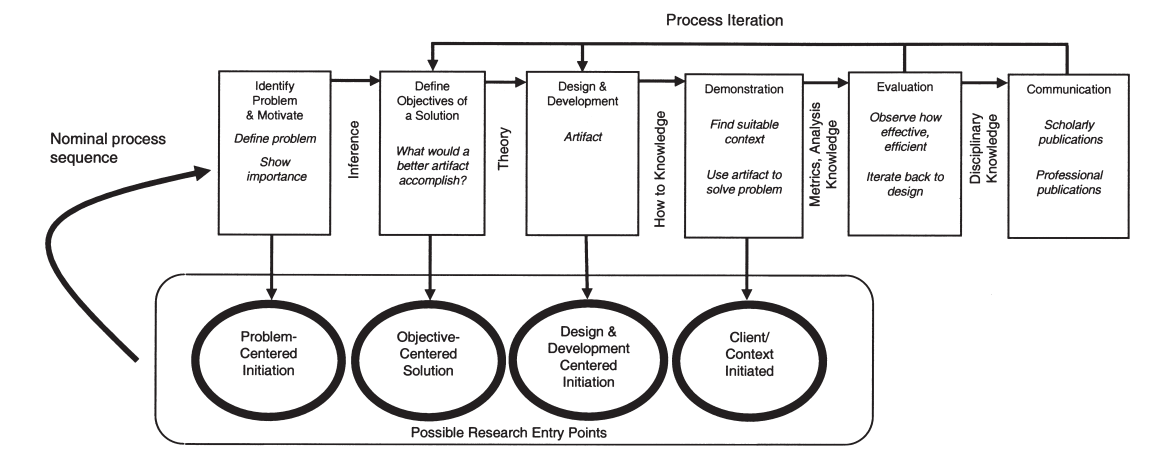
\includegraphics[width=12cm]{images/peffers_dsr_model.png}
	\centering
	\caption{DSR Modell nach Peffers ~\citep{K.Peffers.2007}}
\end{figure}

Bei diesem Modell gibt es mehrere Einstiegsmöglichkeiten (siehe \textit{Possible Research Entry Points}). Der Einstiegspunkt für die vorliegende Arbeit bildet der Punkt \textbf{Problem-Centered Initiation}. Das Problem, welches gelöst werden soll, ist die die starre Natur bestehender Corona Dashboards. Diese Dashboards lassen sich nach \textbf{der Erstellung für die angesprochene Zielgruppe} nur eingeschränkt anpassen oder personalisieren. In diesem Kontext ist die Entwicklung eines Prototyps interessant, welcher die Erstellung der Dashboards \textbf{in die Hände der Zielgruppe selbst legt} und so auch Personalisierungs- und Anpassungsmöglichkeiten bietet. Dies bildet somit die Grundlage für den ersten Schritt des Models \textit{Identify Problem und Motivation}. Im zweiten Schritt \textit{Define Objective of a Solution} geht es darum, das Ziel einer möglichen Lösung aufzuzeigen. Anschliessend geht es im Schritt \textit{Design und Development} um die eigentliche Erstellung des Artefakts, was im Zuge dieser Arbeit ein High Fidelity Prototyp darstellt. Anschliessend geht es in den nächsten Schritten noch um die Evaluation des erstellten Prototyps, sowie die Publikation der Ergebnisse. Jedoch beschränkt sich die vorliegende Arbeit auf die Erstellung eines Prototyps aufgrund teilstrukturierter Interviews mit Millennials. Die eigentliche Evaluation des Prototyps kann im Rahmen einer weiterführenden Arbeit evaluiert werden.


\clearpage
\section{Webbasierte Corona Dashboards}

\subsection{Dashboard – Ein Begriff mit Ursprung in der Automobilindustrie}
    Dashboard bedeutet übersetzt \textit{Armaturenbrett}. Hiermit ist das Armaturenbrett beim Auto gemeint ~\citep{Duden.18.04.2022}. Die Hauptfunktion des Armaturenbrett besteht darin, alle notwendigen Informationen wie Geschwindigkeit, Kilometerzähler etc. schnell und einfach auf einen Blick zu visualisieren. Im Kontext dieser Arbeit wird unter dem Begriff Dashboard die Definition von Duden verwendet. Duden definiert ein Dashboard als: \textbf{Ein Computerprogramm das relevante Informationen zusammenfasst und übersichtlich darstellt} ~\citep{Duden.18.04.2022}. gemeint.


\subsection{Aufbau und Komponenten von webbasierten Dashboards}
Webbasierte Dashboards sind Dashboards, welche über das Internet zugänglich gemacht werden und mit Hilfe eines Webbrowsers dargestellt werden können. Wie herkömmliche Webseiten funktionieren auch webbasierte Dashboards nach dem \textit{Client-Server-Modell} (siehe Abbildung 6). Hierbei sendet der Browser (PC, Smartphone etc.) beim Besuch einer Internet Seite (\url{https://www.covid19.admin.ch/en/overview}) eine Anfrage an den Web Server. Dieser wiederum Antwortet mit dem gewünschten Inhalt (Corona Dashboard). Jedoch benötigt es noch eine dritte, sehr zentrale Komponente, die Datenquelle. In der heutigen Zeit sind Internet Seiten keine starren Textkonstrukte mehr, sie passen sich dynamisch an die Anforderungen des Nutzers an. Besonders für webbasierte Corona Dashboards sind dynamische Daten von enormer Bedeutung. 

Grundsätzlich wird für webbasierte Dashboards mindestens folgende Komponenten benötigt:
\begin{itemize}
    \item Web Server auf welchem die eigentliche Web Applikation läuft und welcher Anfragen entgegennimmt
    \item Datenbank auf welcher die Daten vorhanden sind
    \item Schnittstelle zwischen Datenbank und Webserver, welche die Kommunikation dieser beiden Komponenten ermöglicht
\end{itemize}

\subsection{Vorteile}

Ein grosser Vorteil von webbasierten Dashboards besteht in der grossen Erreichbarkeit der Nutzer. In der heutigen Zeit besitzen die meisten Personen nebst einem Computer ebenfalls über ein Smartphone mit integriertem Browser. Somit ist der Zugriff auf ein webbasiertes Dashboard nebst dem Computer auch über das Smartphone, über ein Tablet etc. möglich. Dies ist von enormer Bedeutung, da man so ortsunabhängig immer auf dem aktuellen Stand ist. Auch können moderne Web Applikationen Gebrauch vom GPS System des Smartphones machen und so standortbezogene Daten liefern. Die Voraussetzung hierzu ist lediglich die Nutzung eines modernen Browsers.

\begin{figure}[ht]
	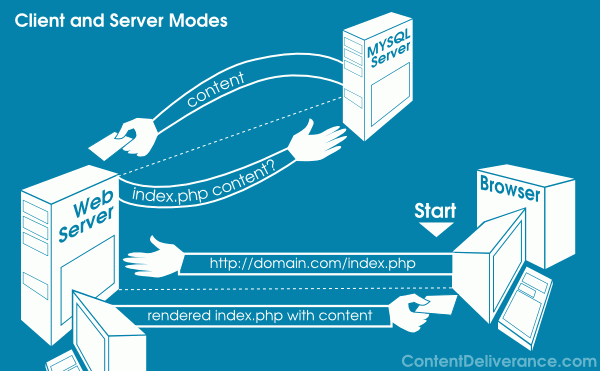
\includegraphics[width=12cm]{images/client_server_model.png}
	\centering
	\caption{Client-Server-Modell ~\citep{client_server_model}}
\end{figure}

\clearpage
\section{Problemidentifizierung und Motivation von webbasierten Corona Dashboards}
Gemäss Peffers soll der Schritt \textit{Problem Identification and Motivation} dabei helfen, den Nutzen einer möglichen Lösung aufzuzeigen. Dies wiederum steigert zum einen die Motivation an der Arbeit selbst und sorgt zum anderen dafür, dass die Beweggründe für alle beteiligten Personen verständlich sind ~\citep[S. 52 + 55]{K.Peffers.2007}.


\subsection{Problemidentifikation}
Als Grundlage für die Problemidentifikation von webbasierten Corona Dashboards dient die Studie von Barbazza. Die Studie erhob die Erfahrungen und Eindrücke von 33 verschiedenen Teams im europäischen Raum, welche für die Konzeption und Umsetzung von Corona Dashboards verantwortlich waren. Im Rahmen der Studie wurden rund 80 Personen aus den 33 Teams befragt. Mit Hilfe von qualitativ durchgeführten Interviews wurden anschliessend verschiedene Kategoriesysteme gebildet. Im Kategoriesystem \textit{Nutzer} fallen folgende Problematiken auf ~\citep[S. 14 + 15]{Barbazza.}:
\begin{itemize}
    \item Keine Definierung einer dedizierten Zielgruppe für Dashboards, Dashboards wurden mehrheitlich für die breite Öffentlichkeit etc. konzipiert
    \item Limitierte Auffassung über den Informationsbedarf der Zielgruppe, kein systematischer Weg um an Nutzer Feedback zu gelangen
\end{itemize}

\subsection{Motivation – Erstellung eines personalisierbaren Corona Dashboards für Millennials}
Das Ziel dieser Arbeit ist die Konzeption und Erstellung eines Corona Dashboards für die Zielgruppe Millennials. Hierbei soll konkret ermittelt werden, welche Informationen sowie Visualisierungsarten für die Zielgruppe von Relevanz sind. Zudem soll ein besonderer Aspekt auf die Anpassbarkeit (Personalisierbarkeit) des Corona Dashboards gelegt werden. Die Lösung soll dazu dienen, den Erstellungsprozess von Dashboards in die Hände der Zielgruppe selbst zu legen. Nutzer können hierbei aus einem Katalog von Visualisierungen auswählen und ihr ganz persönliches Dashboard gestalten. Das erstellte Dashboard kann anschliessend an die relevanten Behörden (BAG) gesendet werden und soll so neue Ideen für Dashboard Designs antreiben sowie das Einholen von Feedback fördern.

\clearpage
\section{Identifikation der Ziele}
TODO

\subsection{Erstellung des Untersuchungsinstrumentes}
TODO

\subsection{Evaluation von Visualisierungstypen für Corona Dashboards}
TODO

\subsection{Identifikation von relevanten Personalisierungsmöglichkeiten in Bezug auf Dashboards}
TODO

\clearpage
\section{Design und Development}
TODO

\subsection{Design mittels Sketching}
TODO

\subsection{High-Fidelity Prototyp als Web Applikation}
TODO

\clearpage
\section{Auswertung}
TODO

\clearpage
\section{Fazit}
TODO

\clearpage
\section{Reflexion und Limitationen}
TODO


\clearpage
\bibliographystyle{apacite}
\urlstyle{rm}
\bibliography{main.bib}

\clearpage
\section*{Anhang}
\begin{table}[ht]
	\begin{tabular}{@{}p{4cm}p{4cm}p{6.5cm}@{}}
		\toprule
		\textbf{Quelle} & \textbf{Schlüsselwörter}        & \textbf{Artikel}        \\ \midrule
		\url{https:                                                                 \\scholar.google.com}                         & covid dashboard                 & ~\citep{Dong.2020}         \\ \midrule
		                &                                 & ~\citep{Florez.2020}    \\ \midrule
		                &                                 & ~\citep{Berry.2020}     \\ \midrule
		                & user centered dashboards        & ~\citep{Francois.2021}  \\ \midrule
		                &                                 & ~\citep{Young.2020}     \\ \midrule
		                & customizable dasbhoards         & ~\citep{Roberts.2017}   \\ \midrule
		\url{https:                                                                 \\dl-acm.org}                                 & covid19 dashboard               & ~\citep{Vitale.}           \\ \midrule
		                & evaluating crisis dashboards    & ~\citep{Ivanov.2018}    \\ \midrule
		                & data dashboards                 & ~\citep{Maheshwari.}    \\ \midrule
		                &                                 & ~\citep{Beheshti.}      \\ \midrule
		\url{https:                                                                 \\google.com}                                 & covid dashboard evaluation      & ~\citep{Barbazza.}         \\ \midrule
		                & how user use covid19 dashboards & ~\citep{Ivankovic.2021} \\ \bottomrule
	\end{tabular}
	\caption{\label{tab:research-protocol}Rechercheprotokoll (Eigene Darstellung)}
\end{table}
\clearpage


\subsection*{Zeitplan}

\begin{table}[ht]
	\begin{tabular}{@{}p{13cm}p{2cm}@{}}
		\toprule
		\textbf{Tätigkeit}                                                                                & \textbf{Stichtag} \\ \midrule
		Erstellung des Untersuchungsinstrumentes                                                          & 08.05.2022        \\ \midrule
		Kapitel Einleitung fertig stellen                                                                 & 08.05.2022        \\ \midrule
		Kapitel Problemidentifizierung und Motivation fertig stellen                                      & 15.05.2022        \\ \midrule
		Durchführung der teilstrukturierten Interviews mit Hilfe des erstellten Untersuchungsinstrumentes & 29.05.2022        \\ \midrule
		Abgabe Exposé                                                                                     & 22.05.2022        \\ \midrule
		Kapitel Identifikation der Ziele fertig stellen                                                   & 05.06.2022        \\ \midrule
		Implementierung Prototyp                                                                          & 26.06.2022        \\ \midrule
		Kapitel Design und Development fertig stellen                                                     & 26.06.2022        \\ \midrule
		Kapitel Fazit fertig stellen                                                                      & 03.07.2022        \\ \midrule
		Kapitel Reflexion und Limitation fertig stellen                                                   & 10.07.2022        \\ \midrule
		Korrekturlesung und Verbesserung                                                                  & 24.07.2022        \\ \midrule
		Abgabe Thesis                                                                                     & 25.07.2022        \\ \bottomrule
	\end{tabular}
	\caption{\label{tab:time-table}Zeitplan (Eigene Darstellung)}
\end{table}

\clearpage
\subsection*{Leitfaden für teilstrukturierte User Interviews}

\subsubsection*{Einleitung}
Als Teil meiner Bachelorarbeit untersuche ich die Konzeption sowie Erstellung eines personalisierbaren Corona-Dashboards für Millennials. Dieses Interview hilft mir dabei drei relevante Fragestellungen in diesem Zusammenhang zu klären. Hierbei ist es wichtig zu erwähnen, dass Sie sich keine Sorgen um korrekte oder inkorrekte Aussagen machen müssen, die besten Antworten sind ihre persönlichen Meinung. Als Erstes sehen wir uns an, welche Informationen in Bezug auf Corona Sie für relevant halten und welche Datenvisualisierungen Sie bevorzugen. Zum Schluss halten wir noch die für Sie wichtigsten Personalisierungsmöglichkeiten fest. Bevor wir jedoch beginnen möchte ich Ihnen noch kurz den Fachbegriff Dashboard erläutern
\\

\textit{Fachbegriff Dashboard}
\\
Der Begriff Dashboard kommt aus der Automobilindustrie und bezeichnet die Frontkonsole (das Dashboard) Ihres Fahrzeugs. Auf dieser sind die wichtigsten Informationen wie Geschwindigkeit, Ölstand etc. auf einen Blick ersichtlich. Dashboards sind also eine Zusammenstellung von verschiedenen Visualisierungen, welche die für Sie relevanten Informationen auf einen Blick ersichtlich machen.\\


\textit{Administrativer Teil}
\\
Kommen wir nun noch kurz zum administrativen Teil. Wie Sie bereits im Vorfeld informiert worden sind, wird dieses Meeting aufgezeichnet. Dies beinhaltet dabei sowohl Ton als auch das Video auf Ihrem Computer. Diese Aufnahmen werden jedoch nicht veröffentlicht, sondern dienen lediglich als Grundlage für Auswertungszwecke im Rahmen dieser Arbeit.\\\\
\textbf{WICHTIG: AUFNAHME STARTEN}


\clearpage
\subsubsection*{Hauptteil}

\textit{Hauptfragen}
\begin{itemize}
    \item Untergeordnete Forschungsfrage 1 und 2 wird via Online Formular beantwortet: \url{https://forms.gle/JdErDGAQ2YkwPZe57}
    \item Untergeordnete Forschungsfrage 3 wird mittels think-aloud Ansatz beantwortet, hierbei wird der Nutzer aufgefordert folgendes Dashboard zu besuchen \url{https://www.covid19.admin.ch/de/overview}
    \begin{itemize}
        \item Was hat Ihnen an diesem Dashboard gefallen?
        \item Was hat Ihnen an diesem Dashboard nicht gefallen?
        \item Was würden Sie sich von diesem Dashboard persönlich wünschen?
        \item Welche Visualisierungen haben Ihnen besonders gefallen und warum?
        \item Gibt es noch andere Visualisierungen welche Sie noch ergänzen möchten (Twitter Feed, Corona Richtlinien in der unmittelbahren Umgebung via GPS)?
        \item Würden Sie es bevorzugen, wenn Sie selbst ein eigenes Dashboard kreieren könnten, sprich eigene Visualisierungen hinzuzufügen?
        \item Ist es Ihnen wichtig, dass Design an Ihre eigenen Bedürfnisse anpassen zu können?
        \item (Nur wenn Anpassung Design wichtig) Welche Aspekte des Designs wollen Sie anpassen können (Farbgebung, Schrift, Titel der Visualisierungen)?
        \item Würden Sie ein leeres Dashboard bevorzugen, auf welchem Sie Ihre eigenen Visualisierungen platzieren können?
        \item Wünschen Sie sich Vorlagen, bzw. Vorschläge von bereits fertig gestellten Dashboards für bestimmte Zwecke (zum Beispiel Über den Schweregrad der Pandemie informieren)?
        \item Sind Ihnen Filterfunktionalitäten wichtig, wenn ja welche (Region, Zeit etc.)?
        \item Würden Sie gerne die Visualisierungen mit Freunden teilen können?
        \item Würden Sie eher eine Desktop Applikation, eine Website oder eine App bevorzugen und warum?
        \item Hätten Sie persönlich Interesste, an der Evaluation eines solchen Prototypen teilzunehmen?
    \end{itemize}
\end{itemize}


\subsubsection*{Schlussteil}
\begin{itemize}
    \item Wünschen Sie noch etwas zu ergänzen oder etwas mitzuteilen?
\end{itemize}

\textbf{WICHTIG: EINWILLIGUNGSERKLÄRUNG PER E-MAIL SENDEN}

\clearpage
\section*{Eigenständigkeitserklärung}
Hiermit bestätigt der Verfasser, dass die vorliegende Arbeit selbstständig verfasst und keine anderen als die angegebenen Hilfsmittel benutzt wurden. Stellen der Arbeit, die dem Wortlaut oder dem Sinn nach anderen Werken entnommen sind, wurden unter Angaben der Quelle kenntlich gemacht.

\begin{figure}[ht]
	
\includegraphics[width=6cm]{images/signature.png}
\end{figure}
Yannick Hutter, Mels am 01. Mai 2022

\end{document}